\documentclass[twoside]{book}

% Packages required by doxygen
\usepackage{fixltx2e}
\usepackage{calc}
\usepackage{doxygen}
\usepackage[export]{adjustbox} % also loads graphicx
\usepackage{graphicx}
\usepackage[utf8]{inputenc}
\usepackage{makeidx}
\usepackage{multicol}
\usepackage{multirow}
\PassOptionsToPackage{warn}{textcomp}
\usepackage{textcomp}
\usepackage[nointegrals]{wasysym}
\usepackage[table]{xcolor}

% Font selection
\usepackage[T1]{fontenc}
\usepackage[scaled=.90]{helvet}
\usepackage{courier}
\usepackage{amssymb}
\usepackage{sectsty}
\renewcommand{\familydefault}{\sfdefault}
\allsectionsfont{%
  \fontseries{bc}\selectfont%
  \color{darkgray}%
}
\renewcommand{\DoxyLabelFont}{%
  \fontseries{bc}\selectfont%
  \color{darkgray}%
}
\newcommand{\+}{\discretionary{\mbox{\scriptsize$\hookleftarrow$}}{}{}}

% Page & text layout
\usepackage{geometry}
\geometry{%
  a4paper,%
  top=2.5cm,%
  bottom=2.5cm,%
  left=2.5cm,%
  right=2.5cm%
}
\tolerance=750
\hfuzz=15pt
\hbadness=750
\setlength{\emergencystretch}{15pt}
\setlength{\parindent}{0cm}
\setlength{\parskip}{3ex plus 2ex minus 2ex}
\makeatletter
\renewcommand{\paragraph}{%
  \@startsection{paragraph}{4}{0ex}{-1.0ex}{1.0ex}{%
    \normalfont\normalsize\bfseries\SS@parafont%
  }%
}
\renewcommand{\subparagraph}{%
  \@startsection{subparagraph}{5}{0ex}{-1.0ex}{1.0ex}{%
    \normalfont\normalsize\bfseries\SS@subparafont%
  }%
}
\makeatother

% Headers & footers
\usepackage{fancyhdr}
\pagestyle{fancyplain}
\fancyhead[LE]{\fancyplain{}{\bfseries\thepage}}
\fancyhead[CE]{\fancyplain{}{}}
\fancyhead[RE]{\fancyplain{}{\bfseries\leftmark}}
\fancyhead[LO]{\fancyplain{}{\bfseries\rightmark}}
\fancyhead[CO]{\fancyplain{}{}}
\fancyhead[RO]{\fancyplain{}{\bfseries\thepage}}
\fancyfoot[LE]{\fancyplain{}{}}
\fancyfoot[CE]{\fancyplain{}{}}
\fancyfoot[RE]{\fancyplain{}{\bfseries\scriptsize Generated by Doxygen }}
\fancyfoot[LO]{\fancyplain{}{\bfseries\scriptsize Generated by Doxygen }}
\fancyfoot[CO]{\fancyplain{}{}}
\fancyfoot[RO]{\fancyplain{}{}}
\renewcommand{\footrulewidth}{0.4pt}
\renewcommand{\chaptermark}[1]{%
  \markboth{#1}{}%
}
\renewcommand{\sectionmark}[1]{%
  \markright{\thesection\ #1}%
}

% Indices & bibliography
\usepackage{natbib}
\usepackage[titles]{tocloft}
\setcounter{tocdepth}{3}
\setcounter{secnumdepth}{5}
\makeindex

% Hyperlinks (required, but should be loaded last)
\usepackage{ifpdf}
\ifpdf
  \usepackage[pdftex,pagebackref=true]{hyperref}
\else
  \usepackage[ps2pdf,pagebackref=true]{hyperref}
\fi
\hypersetup{%
  colorlinks=true,%
  linkcolor=blue,%
  citecolor=blue,%
  unicode%
}

% Custom commands
\newcommand{\clearemptydoublepage}{%
  \newpage{\pagestyle{empty}\cleardoublepage}%
}

\usepackage{caption}
\captionsetup{labelsep=space,justification=centering,font={bf},singlelinecheck=off,skip=4pt,position=top}

%===== C O N T E N T S =====

\begin{document}

% Titlepage & ToC
\hypersetup{pageanchor=false,
             bookmarksnumbered=true,
             pdfencoding=unicode
            }
\pagenumbering{roman}
\begin{titlepage}
\vspace*{7cm}
\begin{center}%
{\Large My Project }\\
\vspace*{1cm}
{\large Generated by Doxygen 1.8.11}\\
\end{center}
\end{titlepage}
\clearemptydoublepage
\tableofcontents
\clearemptydoublepage
\pagenumbering{arabic}
\hypersetup{pageanchor=true}

%--- Begin generated contents ---
\chapter{File Index}
\section{File List}
Here is a list of all files with brief descriptions\+:\begin{DoxyCompactList}
\item\contentsline{section}{\hyperlink{Lab1_8c}{Lab1.\+c} }{\pageref{Lab1_8c}}{}
\end{DoxyCompactList}

\chapter{File Documentation}
\hypertarget{Calendar_8c}{}\section{Calendar.\+c File Reference}
\label{Calendar_8c}\index{Calendar.\+c@{Calendar.\+c}}
{\ttfamily \#include $<$stdio.\+h$>$}\\*
{\ttfamily \#include $<$stdlib.\+h$>$}\\*
Include dependency graph for Calendar.\+c\+:
\nopagebreak
\begin{figure}[H]
\begin{center}
\leavevmode
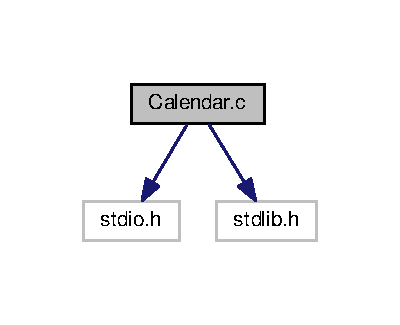
\includegraphics[width=192pt]{Calendar_8c__incl}
\end{center}
\end{figure}
\subsection*{Macros}
\begin{DoxyCompactItemize}
\item 
\#define \hyperlink{Calendar_8c_aa8cecfc5c5c054d2875c03e77b7be15d}{T\+R\+UE}~1
\item 
\#define \hyperlink{Calendar_8c_aa93f0eb578d23995850d61f7d61c55c1}{F\+A\+L\+SE}~0
\end{DoxyCompactItemize}
\subsection*{Functions}
\begin{DoxyCompactItemize}
\item 
int \hyperlink{Calendar_8c_a95952e68642b5c428f757de2469624d6}{get\+\_\+day\+\_\+code} (int year)
\item 
int \hyperlink{Calendar_8c_a66d7a5da36cc9c8ca6085c35c89a3206}{get\+\_\+leap\+\_\+year} (int year)
\item 
void \hyperlink{Calendar_8c_a3db59b9e00ad816835b829f8a7dc56fb}{print\+\_\+calendar} (F\+I\+LE $\ast$fout, int year, int day\+\_\+code, int leap\+\_\+year)
\item 
int \hyperlink{Calendar_8c_a1eeb5dfb948a4386a4c6283c7a9ebcf8}{get\+\_\+year} (void)
\item 
\hyperlink{Calendar_8c_a51af30a60f9f02777c6396b8247e356f}{main} ()
\end{DoxyCompactItemize}


\subsection{Macro Definition Documentation}
\index{Calendar.\+c@{Calendar.\+c}!F\+A\+L\+SE@{F\+A\+L\+SE}}
\index{F\+A\+L\+SE@{F\+A\+L\+SE}!Calendar.\+c@{Calendar.\+c}}
\subsubsection[{\texorpdfstring{F\+A\+L\+SE}{FALSE}}]{\setlength{\rightskip}{0pt plus 5cm}\#define F\+A\+L\+SE~0}\hypertarget{Calendar_8c_aa93f0eb578d23995850d61f7d61c55c1}{}\label{Calendar_8c_aa93f0eb578d23995850d61f7d61c55c1}
\index{Calendar.\+c@{Calendar.\+c}!T\+R\+UE@{T\+R\+UE}}
\index{T\+R\+UE@{T\+R\+UE}!Calendar.\+c@{Calendar.\+c}}
\subsubsection[{\texorpdfstring{T\+R\+UE}{TRUE}}]{\setlength{\rightskip}{0pt plus 5cm}\#define T\+R\+UE~1}\hypertarget{Calendar_8c_aa8cecfc5c5c054d2875c03e77b7be15d}{}\label{Calendar_8c_aa8cecfc5c5c054d2875c03e77b7be15d}


\subsection{Function Documentation}
\index{Calendar.\+c@{Calendar.\+c}!get\+\_\+day\+\_\+code@{get\+\_\+day\+\_\+code}}
\index{get\+\_\+day\+\_\+code@{get\+\_\+day\+\_\+code}!Calendar.\+c@{Calendar.\+c}}
\subsubsection[{\texorpdfstring{get\+\_\+day\+\_\+code(int year)}{get_day_code(int year)}}]{\setlength{\rightskip}{0pt plus 5cm}int get\+\_\+day\+\_\+code (
\begin{DoxyParamCaption}
\item[{int}]{year}
\end{DoxyParamCaption}
)}\hypertarget{Calendar_8c_a95952e68642b5c428f757de2469624d6}{}\label{Calendar_8c_a95952e68642b5c428f757de2469624d6}

\begin{DoxyCode}
45 \{
46 \textcolor{keywordtype}{int} day\_code;
47 \textcolor{keywordtype}{int} x1, x2, x3;
48     x1 = (year - 1.)/ 4.0;
49     x2 = (year - 1.)/ 100.;
50     x3 = (year - 1.)/ 400.;
51 day\_code = (year + x1 - x2 + x3) %7;
52 \textcolor{keywordflow}{return} day\_code;
53 \}             
\end{DoxyCode}
\index{Calendar.\+c@{Calendar.\+c}!get\+\_\+leap\+\_\+year@{get\+\_\+leap\+\_\+year}}
\index{get\+\_\+leap\+\_\+year@{get\+\_\+leap\+\_\+year}!Calendar.\+c@{Calendar.\+c}}
\subsubsection[{\texorpdfstring{get\+\_\+leap\+\_\+year(int year)}{get_leap_year(int year)}}]{\setlength{\rightskip}{0pt plus 5cm}int get\+\_\+leap\+\_\+year (
\begin{DoxyParamCaption}
\item[{int}]{year}
\end{DoxyParamCaption}
)}\hypertarget{Calendar_8c_a66d7a5da36cc9c8ca6085c35c89a3206}{}\label{Calendar_8c_a66d7a5da36cc9c8ca6085c35c89a3206}

\begin{DoxyCode}
55 \{
56     
57 \textcolor{comment}{//if((year% 4) == 0 );}
58 \textcolor{keywordflow}{if}(year% 4==0 && year%100 != 0 || year%400==0)
59    \textcolor{keywordflow}{return} \hyperlink{Calendar_8c_aa8cecfc5c5c054d2875c03e77b7be15d}{TRUE};
60    \textcolor{keywordflow}{else} \textcolor{keywordflow}{return} \hyperlink{Calendar_8c_aa93f0eb578d23995850d61f7d61c55c1}{FALSE};  
61         
62 \}
\end{DoxyCode}
\index{Calendar.\+c@{Calendar.\+c}!get\+\_\+year@{get\+\_\+year}}
\index{get\+\_\+year@{get\+\_\+year}!Calendar.\+c@{Calendar.\+c}}
\subsubsection[{\texorpdfstring{get\+\_\+year(void)}{get_year(void)}}]{\setlength{\rightskip}{0pt plus 5cm}int get\+\_\+year (
\begin{DoxyParamCaption}
\item[{void}]{}
\end{DoxyParamCaption}
)}\hypertarget{Calendar_8c_a1eeb5dfb948a4386a4c6283c7a9ebcf8}{}\label{Calendar_8c_a1eeb5dfb948a4386a4c6283c7a9ebcf8}

\begin{DoxyCode}
38 \{
39 \textcolor{keywordtype}{int} year;
40 printf (\textcolor{stringliteral}{"Enter a year: "});
41 scanf (\textcolor{stringliteral}{"%d"}, &year);
42 \textcolor{keywordflow}{return} year;
43 \}             
\end{DoxyCode}
\index{Calendar.\+c@{Calendar.\+c}!main@{main}}
\index{main@{main}!Calendar.\+c@{Calendar.\+c}}
\subsubsection[{\texorpdfstring{main()}{main()}}]{\setlength{\rightskip}{0pt plus 5cm}main (
\begin{DoxyParamCaption}
{}
\end{DoxyParamCaption}
)}\hypertarget{Calendar_8c_a51af30a60f9f02777c6396b8247e356f}{}\label{Calendar_8c_a51af30a60f9f02777c6396b8247e356f}

\begin{DoxyCode}
15 \{
16    
17    \textcolor{keywordtype}{int} year, day\_code, leap\_year; 
18    
19    FILE *fout;
20    
21    fout = fopen (\textcolor{stringliteral}{"calendar.txt"}, \textcolor{stringliteral}{"w"});
22    
23    year = \hyperlink{Calendar_8c_a1eeb5dfb948a4386a4c6283c7a9ebcf8}{get\_year}();                           
24    
25    day\_code = \hyperlink{Calendar_8c_a95952e68642b5c428f757de2469624d6}{get\_day\_code} (year);
26    
27    leap\_year = \hyperlink{Calendar_8c_a66d7a5da36cc9c8ca6085c35c89a3206}{get\_leap\_year} (year);
28    
29    \hyperlink{Calendar_8c_a3db59b9e00ad816835b829f8a7dc56fb}{print\_calendar}(fout, year, day\_code, leap\_year);
30    
31    printf(\textcolor{stringliteral}{"Open up \(\backslash\)'calendar.txt\(\backslash\)' to see your calendar...\(\backslash\)n"});
32    
33    system(\textcolor{stringliteral}{"pause"});
34      
35 \}
\end{DoxyCode}


Here is the call graph for this function\+:
\nopagebreak
\begin{figure}[H]
\begin{center}
\leavevmode
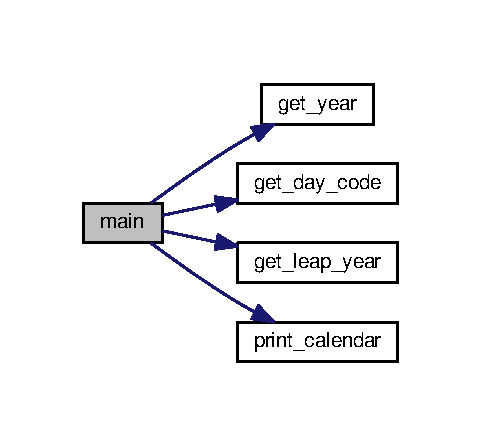
\includegraphics[width=231pt]{Calendar_8c_a51af30a60f9f02777c6396b8247e356f_cgraph}
\end{center}
\end{figure}


\index{Calendar.\+c@{Calendar.\+c}!print\+\_\+calendar@{print\+\_\+calendar}}
\index{print\+\_\+calendar@{print\+\_\+calendar}!Calendar.\+c@{Calendar.\+c}}
\subsubsection[{\texorpdfstring{print\+\_\+calendar(\+F\+I\+L\+E $\ast$fout, int year, int day\+\_\+code, int leap\+\_\+year)}{print_calendar(FILE *fout, int year, int day_code, int leap_year)}}]{\setlength{\rightskip}{0pt plus 5cm}void print\+\_\+calendar (
\begin{DoxyParamCaption}
\item[{F\+I\+LE $\ast$}]{fout, }
\item[{int}]{year, }
\item[{int}]{day\+\_\+code, }
\item[{int}]{leap\+\_\+year}
\end{DoxyParamCaption}
)}\hypertarget{Calendar_8c_a3db59b9e00ad816835b829f8a7dc56fb}{}\label{Calendar_8c_a3db59b9e00ad816835b829f8a7dc56fb}

\begin{DoxyCode}
64 \{
65     \textcolor{keywordtype}{int}  days\_in\_month,     \textcolor{comment}{/* number of days in month currently 
}
66 \textcolor{comment}{                                                     being printed */}
67          day,       \textcolor{comment}{/* counter for day of month */}
68          month;     \textcolor{comment}{/* month = 1 is Jan, month = 2 is Feb, etc. */}
69      fprintf (fout,\textcolor{stringliteral}{"                   %d"}, year);
70      \textcolor{keywordflow}{for} ( month = 1; month <= 12; month++ ) \{
71           \textcolor{keywordflow}{switch} ( month ) \{ \textcolor{comment}{/* print name and set days\_in\_month */}
72           \textcolor{keywordflow}{case} 1:
73                fprintf(fout,\textcolor{stringliteral}{"\(\backslash\)n\(\backslash\)nJanuary"} );
74                days\_in\_month = 31;
75                \textcolor{keywordflow}{break};
76           \textcolor{keywordflow}{case} 2:
77                fprintf(fout,\textcolor{stringliteral}{"\(\backslash\)n\(\backslash\)nFebruary"} );
78                days\_in\_month = leap\_year ? 29 : 28;
79                \textcolor{keywordflow}{break};
80           \textcolor{keywordflow}{case} 3:
81                fprintf(fout, \textcolor{stringliteral}{"\(\backslash\)n\(\backslash\)nMarch"} );
82                days\_in\_month = 31;
83                \textcolor{keywordflow}{break};
84           \textcolor{keywordflow}{case} 4:
85                fprintf(fout,\textcolor{stringliteral}{"\(\backslash\)n\(\backslash\)nApril"} );
86                days\_in\_month = 30;
87                \textcolor{keywordflow}{break};
88           \textcolor{keywordflow}{case} 5:
89                fprintf(fout,\textcolor{stringliteral}{"\(\backslash\)n\(\backslash\)nMay"} );
90                days\_in\_month = 31;
91                \textcolor{keywordflow}{break};
92           \textcolor{keywordflow}{case} 6:
93                fprintf(fout,\textcolor{stringliteral}{"\(\backslash\)n\(\backslash\)nJune"} );
94                days\_in\_month = 30;
95                \textcolor{keywordflow}{break};
96           \textcolor{keywordflow}{case} 7:
97                fprintf(fout,\textcolor{stringliteral}{"\(\backslash\)n\(\backslash\)nJuly"} );
98                days\_in\_month = 31;
99                \textcolor{keywordflow}{break};
100           \textcolor{keywordflow}{case} 8:
101                fprintf(fout,\textcolor{stringliteral}{"\(\backslash\)n\(\backslash\)nAugust"} );
102                days\_in\_month = 31;
103                \textcolor{keywordflow}{break};
104           \textcolor{keywordflow}{case} 9:
105                fprintf(fout,\textcolor{stringliteral}{"\(\backslash\)n\(\backslash\)nSeptember"} );
106                days\_in\_month = 30;
107                \textcolor{keywordflow}{break};
108           \textcolor{keywordflow}{case} 10:
109                fprintf(fout,\textcolor{stringliteral}{"\(\backslash\)n\(\backslash\)nOctober"} );
110                days\_in\_month = 31;
111                \textcolor{keywordflow}{break};
112           \textcolor{keywordflow}{case} 11:
113                fprintf(fout,\textcolor{stringliteral}{"\(\backslash\)n\(\backslash\)nNovember"} );
114                days\_in\_month = 30;
115                \textcolor{keywordflow}{break};
116           \textcolor{keywordflow}{case} 12:
117                fprintf(fout,\textcolor{stringliteral}{"\(\backslash\)n\(\backslash\)nDecember"} );
118                days\_in\_month = 31;
119                \textcolor{keywordflow}{break};
120           \}
121           fprintf(fout,\textcolor{stringliteral}{"\(\backslash\)n\(\backslash\)nSun  Mon  Tue  Wed  Thu  Fri  Sat\(\backslash\)n"} );
122           \textcolor{comment}{/* advance printer to correct position for first date */}
123           \textcolor{keywordflow}{for} ( day = 1; day <= 1 + day\_code * 5; day++ )
124                fprintf(fout,\textcolor{stringliteral}{" "} );
125           \textcolor{comment}{/* print the dates for one month */}
126           \textcolor{keywordflow}{for} ( day = 1; day <= days\_in\_month; day++ ) \{
127                fprintf(fout,\textcolor{stringliteral}{"%2d"}, day );
128                \textcolor{keywordflow}{if} ( ( day + day\_code ) % 7 > 0 ) \textcolor{comment}{/* before Sat? */}
129                     \textcolor{comment}{/* move to next day in same week */}
130                     fprintf(fout,\textcolor{stringliteral}{"   "} );
131                \textcolor{keywordflow}{else}  \textcolor{comment}{/* skip to next line to start with Sun */}
132                     fprintf(fout, \textcolor{stringliteral}{"\(\backslash\)n "} );
133           \}
134           \textcolor{comment}{/* set day\_code for next month to begin */}
135           day\_code = ( day\_code + days\_in\_month ) % 7;
136      \}
137 \}\end{DoxyCode}

%--- End generated contents ---

% Index
\backmatter
\newpage
\phantomsection
\clearemptydoublepage
\addcontentsline{toc}{chapter}{Index}
\printindex

\end{document}
